\documentclass[xcolor=dvipsnames]{beamer}

\usepackage{amsmath, amssymb, graphicx}
\usepackage[english]{babel}
\usepackage{times}
\usepackage[utf8]{inputenc}
\usepackage[T1]{fontenc}
\usepackage{listings}
\usepackage[norelsize,ruled,vlined]{algorithm2e}
\usepackage{color}
\usepackage{hyperref}
\usepackage{listings}
\usepackage{booktabs}
\usepackage{listings}
\usepackage{tikz}
\usepackage{xcolor}
\usepackage{caption}
\usetikzlibrary{matrix}
\usetikzlibrary{arrows}
\usetikzlibrary{positioning}
\usetikzlibrary{shapes.multipart}

\theoremstyle{definition}
\newtheorem{proposition}{Proposition}
\DeclareCaptionFont{white}{\color{white}}
\DeclareCaptionFormat{listing}{\colorbox[cmyk]{0.43, 0.35, 0.35,0.01}{\parbox{\textwidth}{\hspace{15pt}#1#2#3} } }
\captionsetup[lstlisting]{format=listing, labelfont=white, textfont=white, singlelinecheck=false, margin=0pt, font={bf,footnotesize} }

\newcommand{\fancyh}{\mathcal{H}}
\newcommand{\gangle}[1]{\langle{} #1 \rangle{}}
\newcommand{\myd}{\mathrm{d}}
\newcommand{\NN}{\mathbb{N}}
\newcommand{\RR}{\mathbb{R}}
\newcommand{\ZZ}{\mathbb{Z}}

\definecolor{dkgreen}{rgb}{0,0.6,0}
\definecolor{gray}{rgb}{0.5,0.5,0.5}
\definecolor{mauve}{rgb}{0.58,0,0.82}

\lstset{language=Scala,
  aboveskip=3mm,
  basicstyle={\normalsize\ttfamily},
  belowskip=3mm,
  gobble=20,
  breakatwhitespace=true,
  breaklines=true,
  columns=flexible,
  commentstyle=\color{dkgreen},
  keywordstyle=\color{blue},
  numbers=none,
  numberstyle=\tiny\color{gray},
  showstringspaces=false,
  stepnumber=1,
  stringstyle=\color{mauve},
  tabsize=2,
}



\mode<presentation>
{\setbeamertemplate{navigation symbols}{}
    \setbeamertemplate{items}[ball]
    % \setbeamertemplate{blocks}[rounded][shadow=true]
    \beamertemplatenavigationsymbolsempty
    \usecolortheme[named=Sepia]{structure}
    \usetheme{Warsaw}
    \useoutertheme{infolines}
    \setbeamercovered{transparent}
}

\definecolor{mygreen}{rgb}{0, 178, 115}

\tikzstyle{block} = [rectangle, draw, font=\tiny, text centered, rounded corners, minimum height=1em, node distance=1.5cm, minimum width=2em]
\tikzstyle{line} = [draw, -latex']
\tikzstyle{value} = [label, black, font=\tiny, thick, node distance=0.4cm]

\title[Directembedding]{Directembedding \\ {\small Concealing the Deep Embedding of DSLs}}
\author{Ólafur Páll Geirsson}
% \department{School of Computer and Communication Sciences}
% \project{Semester Project}
\institute[EPFL]{École Polytechnique Fédérale de Lausanne \\
    School of Computer and Communication Sciences\\
\logoepfl}
\date{\today}


% Delete this, if you do not want the table of contents to pop up at
% the beginning of each subsection:
\AtBeginSection[]
{\begin{frame}<beamer>{Overview}
        \tableofcontents[
            sections={1-6},
            currentsection,
            currentsubsection,
            hideothersubsections,
            sectionstyle=show/shaded,
        subsectionstyle=show/shaded/hide]
    \end{frame}
}

\begin{document}

\newcommand{\logoepfl}[0]{\begin{center}
    
\includegraphics[width=2cm]{logo_epfl_coul.eps}
    \vspace{-0.5cm}
  \end{center}
}


%%%%%%%%%%%%%%%%%%%%%%%%%%%%%%%%%%%%%%%%%%%%%%%%%%%%%%%%%%%%%%%
% 0. Titlepage
%%%%%%%%%%%%%%%%%%%%%%%%%%%%%%%%%%%%%%%%%%%%%%%%%%%%%%%%%%%%%%%
\begin{frame}
    \titlepage{}
\end{frame}
% \begin{frame}{Today's agenda}
% \tableofcontents[hideallsubsections,
%     sections={1-6}
% ]
% \end{frame}

%%%%%%%%%%%%%%%%%%%%%%%%%%%%%%%%%%%%%%%%%%%%%%%%%%%%%%%%%%%%%%%
% 1. Motivation
%%%%%%%%%%%%%%%%%%%%%%%%%%%%%%%%%%%%%%%%%%%%%%%%%%%%%%%%%%%%%%%
\section{Motivation} % (fold)
\label{sec:Motivation}
\begin{frame}[fragile]
    \frametitle{Motivation}
    \begin{block}{Mission statement}
        Enable wider adoption of embedded DSLs
    \end{block}
\end{frame}

\begin{frame}[fragile]
    \frametitle{The Struggle}
    \framesubtitle{Deeply embedded vs. Shallowly embedded}
    % \begin{block}{DSL Author}
    %     Possible expert, wants full control over DSL behaviour
    % \end{block}
    % \begin{block}{DSL User}
    %     Possible beginner, wants user-friendly interface
    % \end{block}
    \huge
    \begin{center}
        \begin{tabular}{lcc}
                    & Author & User   \\
            Deep    &   
\includegraphics[width=1cm]{img/happy.png}   & 
\includegraphics[width=1cm]{img/sad.png}    \\
            Shallow &   
\includegraphics[width=1cm]{img/sad.png}     & 
\includegraphics[width=1cm]{img/happy.png}  \\
        \end{tabular}
    \end{center}
\end{frame}


%%%%%%%%%%%%%%%%%%%%%%%%%%%%%%%%%%%%%%%%%%%%%%%%%%%%%%%%%%%%%%%
% 2. Directembedding
%%%%%%%%%%%%%%%%%%%%%%%%%%%%%%%%%%%%%%%%%%%%%%%%%%%%%%%%%%%%%%%
% subsection Motivation (end)
\section{Directembedding} % (fold)
\label{sec:Directembedding}

\subsection{Architecture} % (fold)
\label{sub:Architecture}

\begin{frame}[fragile]
    \frametitle{Pipeline}
    \begin{center}
        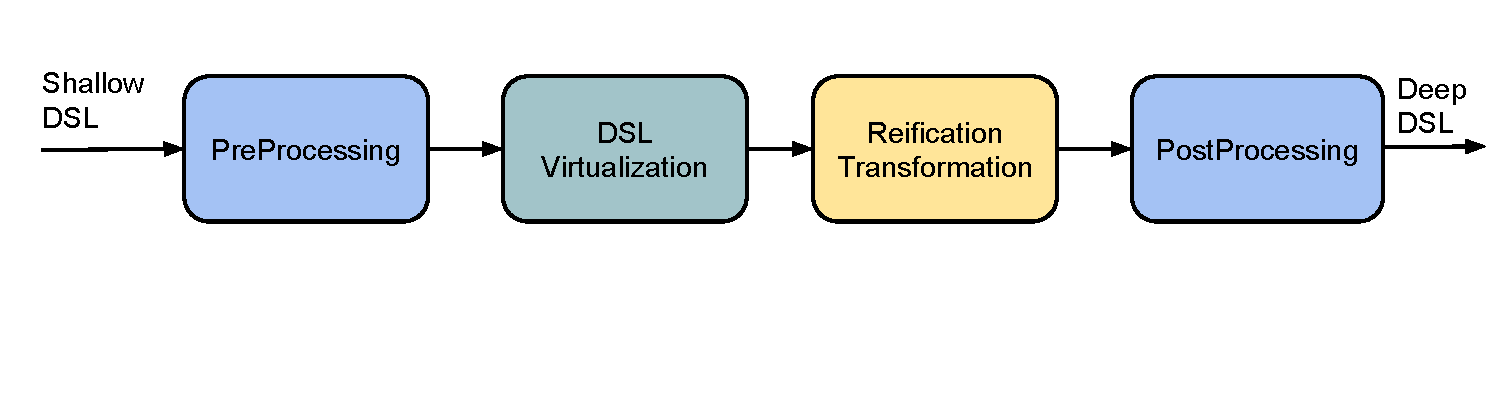
\includegraphics[width=\textwidth]{img/Architecture.pdf}
    \end{center}
\end{frame}

% subsection Architecture (end)

\subsection{Language virtualization} % (fold)
\label{sub:Languagevirtualization}
\begin{frame}[fragile]
    \frametitle{Language Virtualization}
    \begin{block}{Override standard language features}
        \lstinputlisting{code/language-virtualization.scala}
    \end{block}
\end{frame}

% subsection Language virtualization (end)

\subsection{Type overriding} % (fold)
\label{sub:Typeoverriding}

\begin{frame}[fragile]
    \frametitle{Type overriding}
    \begin{block}{Override behavior predefined and third-party types}
        \lstinputlisting{code/type-overriding.scala}
    \end{block}
\end{frame}

% subsection Type overriding (end)

\subsection{Improved error messages} % (fold)
\label{sub:Improvederrormessages}
\begin{frame}[fragile]
    \frametitle{Improved error messages}
    \begin{block}{}
        \lstinputlisting{code/errors.scala}
    \end{block}
\end{frame}

% subsection Improved error messages (end)

\subsection{Configuration} % (fold)
\label{sub:Directembeddingconfiguration}
\begin{frame}[fragile]
    \frametitle{Configuration}
    \framesubtitle{@reifyAs}
    \begin{block}{}
        \lstinputlisting{../report/code/reifyAs.scala}
    \end{block}
\end{frame}

\begin{frame}[fragile]
    \frametitle{Configuration}
    \framesubtitle{@reifyAsInvoked}
    \begin{block}{}
        \lstinputlisting{../report/code/reifyAsInvoked.scala}
    \end{block}
\end{frame}

\begin{frame}[fragile]
    \frametitle{Configuration}
    \framesubtitle{@passThrough}
    \begin{block}{}
        \lstinputlisting{../report/code/passThrough.scala}
    \end{block}
\end{frame}
% subsection configuration (end)



%%%%%%%%%%%%%%%%%%%%%%%%%%%%%%%%%%%%%%%%%%%%%%%%%%%%%%%%%%%%%%%
% 3. Slick-direct
%%%%%%%%%%%%%%%%%%%%%%%%%%%%%%%%%%%%%%%%%%%%%%%%%%%%%%%%%%%%%%%
% subsection Motivation (end)
\section{Case study: slick-direct v2} % (fold)
\label{sec:Slick-direct}

\begin{frame}[fragile]
    \frametitle{Problem statement}
    \begin{block}{Problem statement}
        Develop an awesome embedded query language in Scala
    \end{block}
\end{frame}

\subsection{Lifted embedding} % (fold)
\label{sub:Liftedembedding}

\begin{frame}[fragile]
    \frametitle{Lifted embedding}
    \framesubtitle{aka Slick}
    \begin{itemize}
        \item Currently supported API in Slick 3.0
    \end{itemize}
    \begin{block}{The good parts}
        \begin{enumerate}
            \item Uses standard Scala
            \item Feature rich
        \end{enumerate}
    \end{block}
    \begin{block}{The bad parts}
        \begin{enumerate}
            \item Lifted embedding table requires boilerplate
            \item Cryptic error messages
        \end{enumerate}
    \end{block}
\end{frame}

\begin{frame}[fragile]
    \frametitle{Problem 1}
    \framesubtitle{Lifted embedding table requires boilerplate}
    \lstinputlisting{code/boilerplate.scala}
\end{frame}

\begin{frame}[fragile]
    \frametitle{Problem 2}
    \framesubtitle{Cryptic error messages}
    \begin{verbatim}
[Error] User.scala:25: No matching Shape found.
Slick does not know how to map the given types.
Possible causes: T in Table[T] does not
match your * projection.  Or you use an
unsupported type in a Query (e.g. scala List).
  Required level: slick.lifted.FlatShapeLevel
     Source type:
(slick.lifted.Rep[Int], slick.lifted.Rep[String],
    slick.lifted.Rep[Int])
   Unpacked type: (Int, String)
     Packed type: Any
def * = ProvenShape.proveShapeOf(
(id, name, id) <> ((User.apply _).tupled,User.unapply))
                ^
    \end{verbatim}
\end{frame}

% subsection Lifted embedding (end)

\subsection{Direct embedding v1} % (fold)
\label{sub:Directembeddingv1}

\begin{frame}[fragile]
    \frametitle{Direct embedding}
    \framesubtitle{Deprecated in Slick 3.0}
    \begin{block}{The good parts}
        \begin{enumerate}
            \item No more boilerplate
            \item Comprehensible error messages
        \end{enumerate}
    \end{block}
    \begin{block}{The bad parts}
        \begin{enumerate}
            \item Queries can fail at runtime
            \item Difficult to develop and maintain
        \end{enumerate}
    \end{block}
\end{frame}

\begin{frame}[fragile]
    \frametitle{Benefit 1}
    \framesubtitle{No more boilerplate}
    \begin{block}{}
        \lstinputlisting{code/no-more-boilerplate.scala}
    \end{block}
\end{frame}

\begin{frame}[fragile]
    \frametitle{Problem 1}
    \framesubtitle{Queries can fail at runtime}
    \begin{block}{}
        \lstinputlisting{code/runtime-fail.scala}
    \end{block}
\end{frame}

% subsection Direct embedding v1 (end)

\subsection{Shadow embedding} % (fold)
\label{sub:Shadowembedding}
\begin{frame}[fragile]
    \frametitle{Shadow embedding}
    \framesubtitle{Powered by Yin-Yang}
    \begin{itemize}
        \item Master project of Amir Shaikhha, August 2013
    \end{itemize}
    \begin{block}{The good parts}
        \begin{enumerate}
            \item User-friendly API
            \item Comprehensive and comprehensible error messages
            \item Great performance
        \end{enumerate}
    \end{block}
    \begin{block}{The not so good parts}
        \begin{enumerate}
            \item Challenging for the DSL author
        \end{enumerate}
    \end{block}
    \only<1> {
        \vspace{0.5cm}
    }
    \only<2> {
        We are almost there!
    }
\end{frame}

\begin{frame}[fragile]
    \frametitle{Problem}
    \framesubtitle{Auto generated SlickCake}
    \begin{block}{}
        \lstinputlisting{code/slickcake.scala}
    \end{block}
\end{frame}

\begin{frame}[fragile]
    \frametitle{Problem}
    \framesubtitle{3 layers of Query}
    \begin{block}{}
        \lstinputlisting{code/yyquery.scala}
    \end{block}
\end{frame}

% subsection Shadow embedding (end)

\subsection{Direct embedding v2} % (fold)
\label{sub:Direct embedding}

\begin{frame}[fragile]
    \frametitle{Directembedding}
    \framesubtitle{From shallow to deep in one step}
    \begin{center}
        \Huge
        slick-direct v2
    \end{center}
\end{frame}

\begin{frame}[fragile]
    \frametitle{Pipeline reminder}
    \begin{center}
        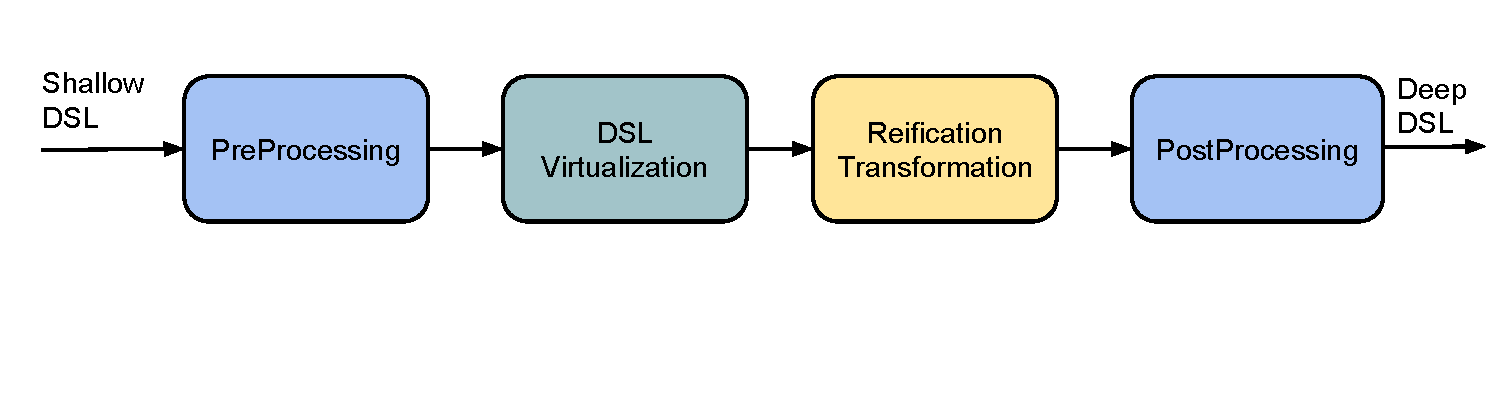
\includegraphics[width=\textwidth]{img/Architecture.pdf}
    \end{center}
\end{frame}

\begin{frame}[fragile]
    \frametitle{Shallow configuration}
    \framesubtitle{Simplified example}
    \begin{block}{}
        \lstinputlisting{code/direct-config.scala}
    \end{block}
\end{frame}

\begin{frame}[fragile]
    \frametitle{Deep configuration}
    \framesubtitle{Simplified example}
    \begin{block}{}
        \lstinputlisting{code/direct-config2.scala}
    \end{block}
\end{frame}


\begin{frame}[fragile]
    \frametitle{Directembedding transformation}
    \framesubtitle{Pipeline}
    \begin{block}{Shallow query}
        \lstinputlisting{code/pipeline1.scala}
    \end{block}
    \begin{center}
        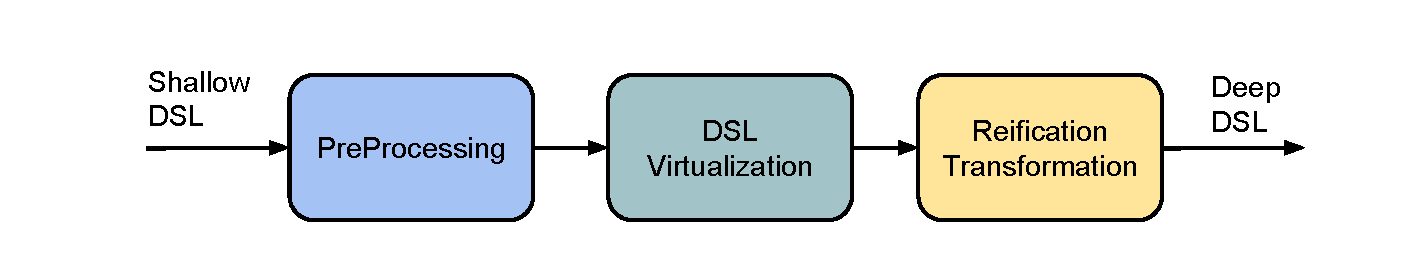
\includegraphics[width=\textwidth]{img/pipeline1.pdf}
    \end{center}
\end{frame}

\begin{frame}[fragile]
    \frametitle{Directembedding transformation}
    \framesubtitle{Pipeline}
    \begin{block}{PreProcessing}
        \lstinputlisting{code/pipeline2.scala}
    \end{block}
    \begin{center}
        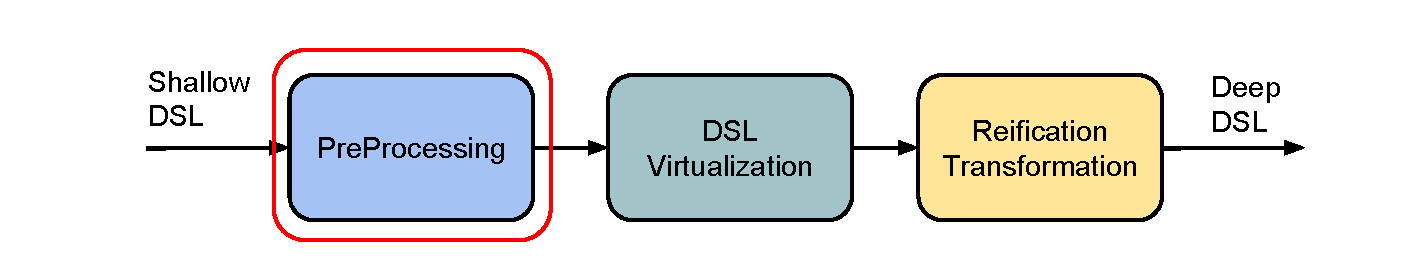
\includegraphics[width=\textwidth]{img/pipeline2.pdf}
    \end{center}
\end{frame}


\begin{frame}[fragile]
    \frametitle{Directembedding transformation}
    \framesubtitle{Pipeline}
    \begin{block}{DSL Virtualization}
        \lstinputlisting{code/pipeline3.scala}
    \end{block}
    \begin{center}
        \vspace{-0.5cm}
        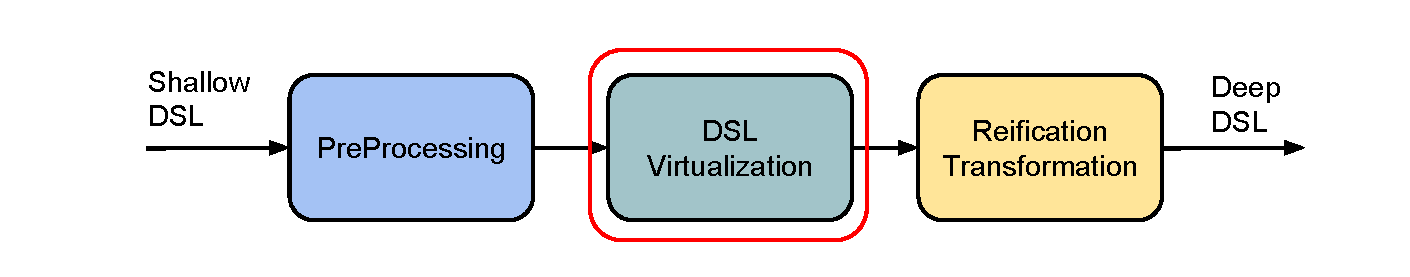
\includegraphics[width=\textwidth]{img/pipeline3.pdf}
    \end{center}
\end{frame}

\begin{frame}[fragile]
    \frametitle{Directembedding transformation}
    \framesubtitle{Pipeline}
    \begin{block}{Reification Transformation}
        \lstinputlisting{code/pipeline4.scala}
    \end{block}
    \begin{center}
        \vspace{-0.5cm}
        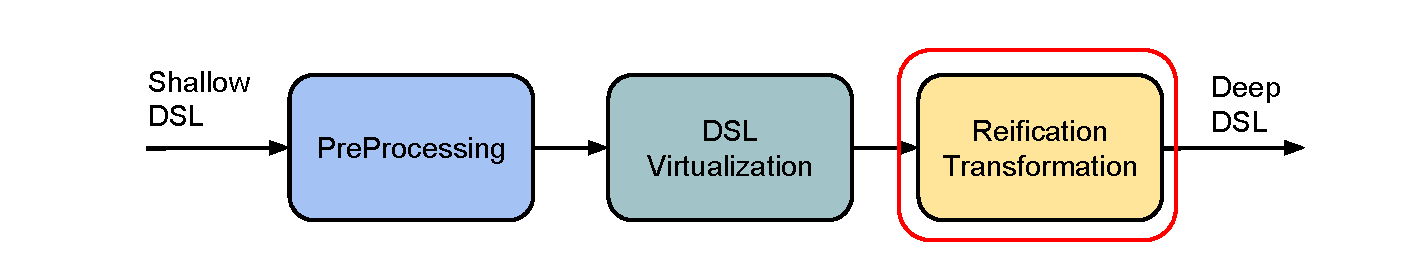
\includegraphics[width=\textwidth]{img/pipeline4.pdf}
    \end{center}
\end{frame}

\begin{frame}[fragile]
    \frametitle{It works!}
    \begin{block}{FilterSpec}
        \lstinputlisting{code/filterspec.scala}
    \end{block}
\end{frame}

% subsection Direct embedding (end)

\section{Conclusion} % (fold)
\label{sec:Conclusion}

\begin{frame}[fragile]
    \frametitle{Conclusion}
    \begin{block}{Directembedding}
        \begin{itemize}
            \item Language virtualization
            \item Type overriding
            \item More reification options
            \item Improved configuration
        \end{itemize}
    \end{block}
    \begin{block}{Slick-direct v2}
        \begin{itemize}
            \item Under 300 LOC, developed in less than 2 weeks
            \item Queries supported: select *, join, filter, map, flatMap, take, (custom column types)
        \end{itemize}
    \end{block}
\end{frame}

\begin{frame}[fragile]
    \frametitle{Future work}
    \begin{itemize}
        \item More case studies
        \item Improve slick-direct
    \end{itemize}
\end{frame}

\begin{frame}[fragile]
    \frametitle{The End}
    \begin{center}
        \Huge
        Thank you!
    \end{center}
\end{frame}

% subsection Evaluation (end)


\end{document}
